\subsection{False rumor early detection}
In this subsection, we evaluate the ability of the hybrid
SVM classifier in detecting false rumors
in the early stage of propagation. Given a detection deadline,
we assume all reposts and related information published after
this deadline are invisible when testing the model of the classifier.
For example, if the detection deadline is 24 hours, then we only use the data
that was generated during the first day after the original message
is posted. The sooner the deadline, the less data of reposts and hence
the propagation structures can be used. A deadline of 0 hours
means that we will not use any repost data except the original messages
themselves. Such detection deadlines affects
the graph kernel as well as all features in REPOST category.

\begin{figure}[htb]
\centering
\includegraphics[height=120pt]{detect_origin.eps}
\caption{False rumor early detection}
\label{fig:early_detection}
\end{figure}

\figref{fig:early_detection} shows the average accuracy of detection
for various deadlines. The experiment was performed on the small
data set. The data set was divided into two parts evenly,
one part was used to learn the model of classifier,
another part was used to test the model.
When learning the model, all training data is used,
while only the test data before the deadline is
used when testing the model.
Our model (Hybrid) achieves 72\% accuracy when deadline is 0.
This accuracy is low because there is no information
of propagation structure but only some static features from
the original messages.
As deadline is lengthened, the accuracy climbs rapidly, which
indicates that the features from the responses and the propagation graph
weigh in. By 24 hours after the initial posting, the detection
accuracy is 88\%, which suggests that the model
is 88\% confident to detect an average false rumors within the first
day of the posting of original messages.
We also experimented with rumor early detection on
Yang's\cite{yang2012automatic} and Castillo's\cite{castillo2011information} 
algorithms, and compare their results with ours in \figref{fig:early_detection}.
The accuracies of the three methods at time 0 are mostly
the same because three methods share similar basic features when
there is no repost. However, after 24 hours, Yang's result improves a little,
Castillo's improves substantially, while ours improves the most.
This is because Yang's method uses only simple features related to reposting
(e.g., ``IS RETWEETED'', ``NUM OF COMMENTS'', ``NUM OF RETWEETES''),
Castillo's method includes some simple but effective features of
reposting such as ``AVG SENTIMENT SCORE'' and ``PROPAGATION MAX LEVEL'',
while our method considers the propagation structure as well as
many other reposting features and thus benefits most from the signals of
the reposts. Among the three methods, ours converges most quickly in terms of
early false rumor detection.
